%\documentclass[5p,times,longtitle,preprint]{elsarticle}
\documentclass[5p,times,preprint]{elsarticle}

\usepackage{amsmath}
\usepackage{amssymb}
\usepackage{soul}

%\usepackage[]{lineno}
%\renewcommand\linenumberfont{\ttfamily\bfseries\tiny}
%\setlength\linenumbersep{5pt}
%\linenumbers

\usepackage{enumerate}
\usepackage{graphicx}% Include figure files
\usepackage{dcolumn}% Align table columns on decimal pion\index{\footnote{}}t
\usepackage{bm}% bold math
\usepackage{color}% bold math

\usepackage{epstopdf}
\usepackage{subcaption}

\hyphenpenalty=1500
\exhyphenpenalty=1500
\journal{Nuclear Instruments and Methods in Physics Research A}
\begin{document}
\begin{frontmatter}
\title{Characterization of Hammamatsu Multianode Photo Multiplier Tubes H8500 and H12700}

\author[A]{P.~Degtiarenko }
\author[B]{A. Kim \corref{cor1}} 
\ead{kenjo@jlab.org}
\cortext[cor1]{ Corresponding author Tel: +1 757 269 6356}
\author[A]{V. Kubarovsky }

\author[C]{A. Smith}

\address[A]{Jefferson Lab, Newport News, Virginia, USA}
\address[B]{University of Connecticut, Storrs, CT 0626, USA}
\address[C]{Duke University, Durham, NC 2770, USA}

\begin{abstract}
%% Text of abstract
Characterization of Hammamatsu Multianode Photo Multiplier Tubes H8500 and H12700.

\end{abstract}

\begin{keyword}
Ring Imaging Cherenkov detector \sep
Multianode Photo Multiplier tubes H8500 and H12700 \sep
Photon detector \sep Photomultiplier  \sep
Photoelectron  \sep  Signal amplitude spectra \sep 
Photon detection efficiency
\end{keyword}


\end{frontmatter}

\section{Introduction}

As part of the ongoing study of the structure of nucleons in Hall B at the Thomas Jefferson National Accelerator Facility (JLab) \cite{Avakian:2012ca}, the CEBAF Large Acceptance Spectrometer (CLAS12) aims to accurately identify the secondary particles of high energy reactions, assist in probing the strangeness frontier, and aid in characterizing transverse momentum distribution (TMD) and generalized parton distribution (GPD) functions. Indispensable to this task is the ability to identify kaons, pions, and protons.  With the CLAS12 spectrometer providing accurate momentum measurements the RICH detector \cite{Contalbrigo:2020,Contalbrigo:2020snw,Mirazita:2017vav,Contalbrigo:2014rqa} provides tandem Cherenkov lightcone radius measurements which yield the velocities of near light-speed particles, thus facilitating mass-dependent particle identification.

\begin{figure}[hbt]
	\centering
	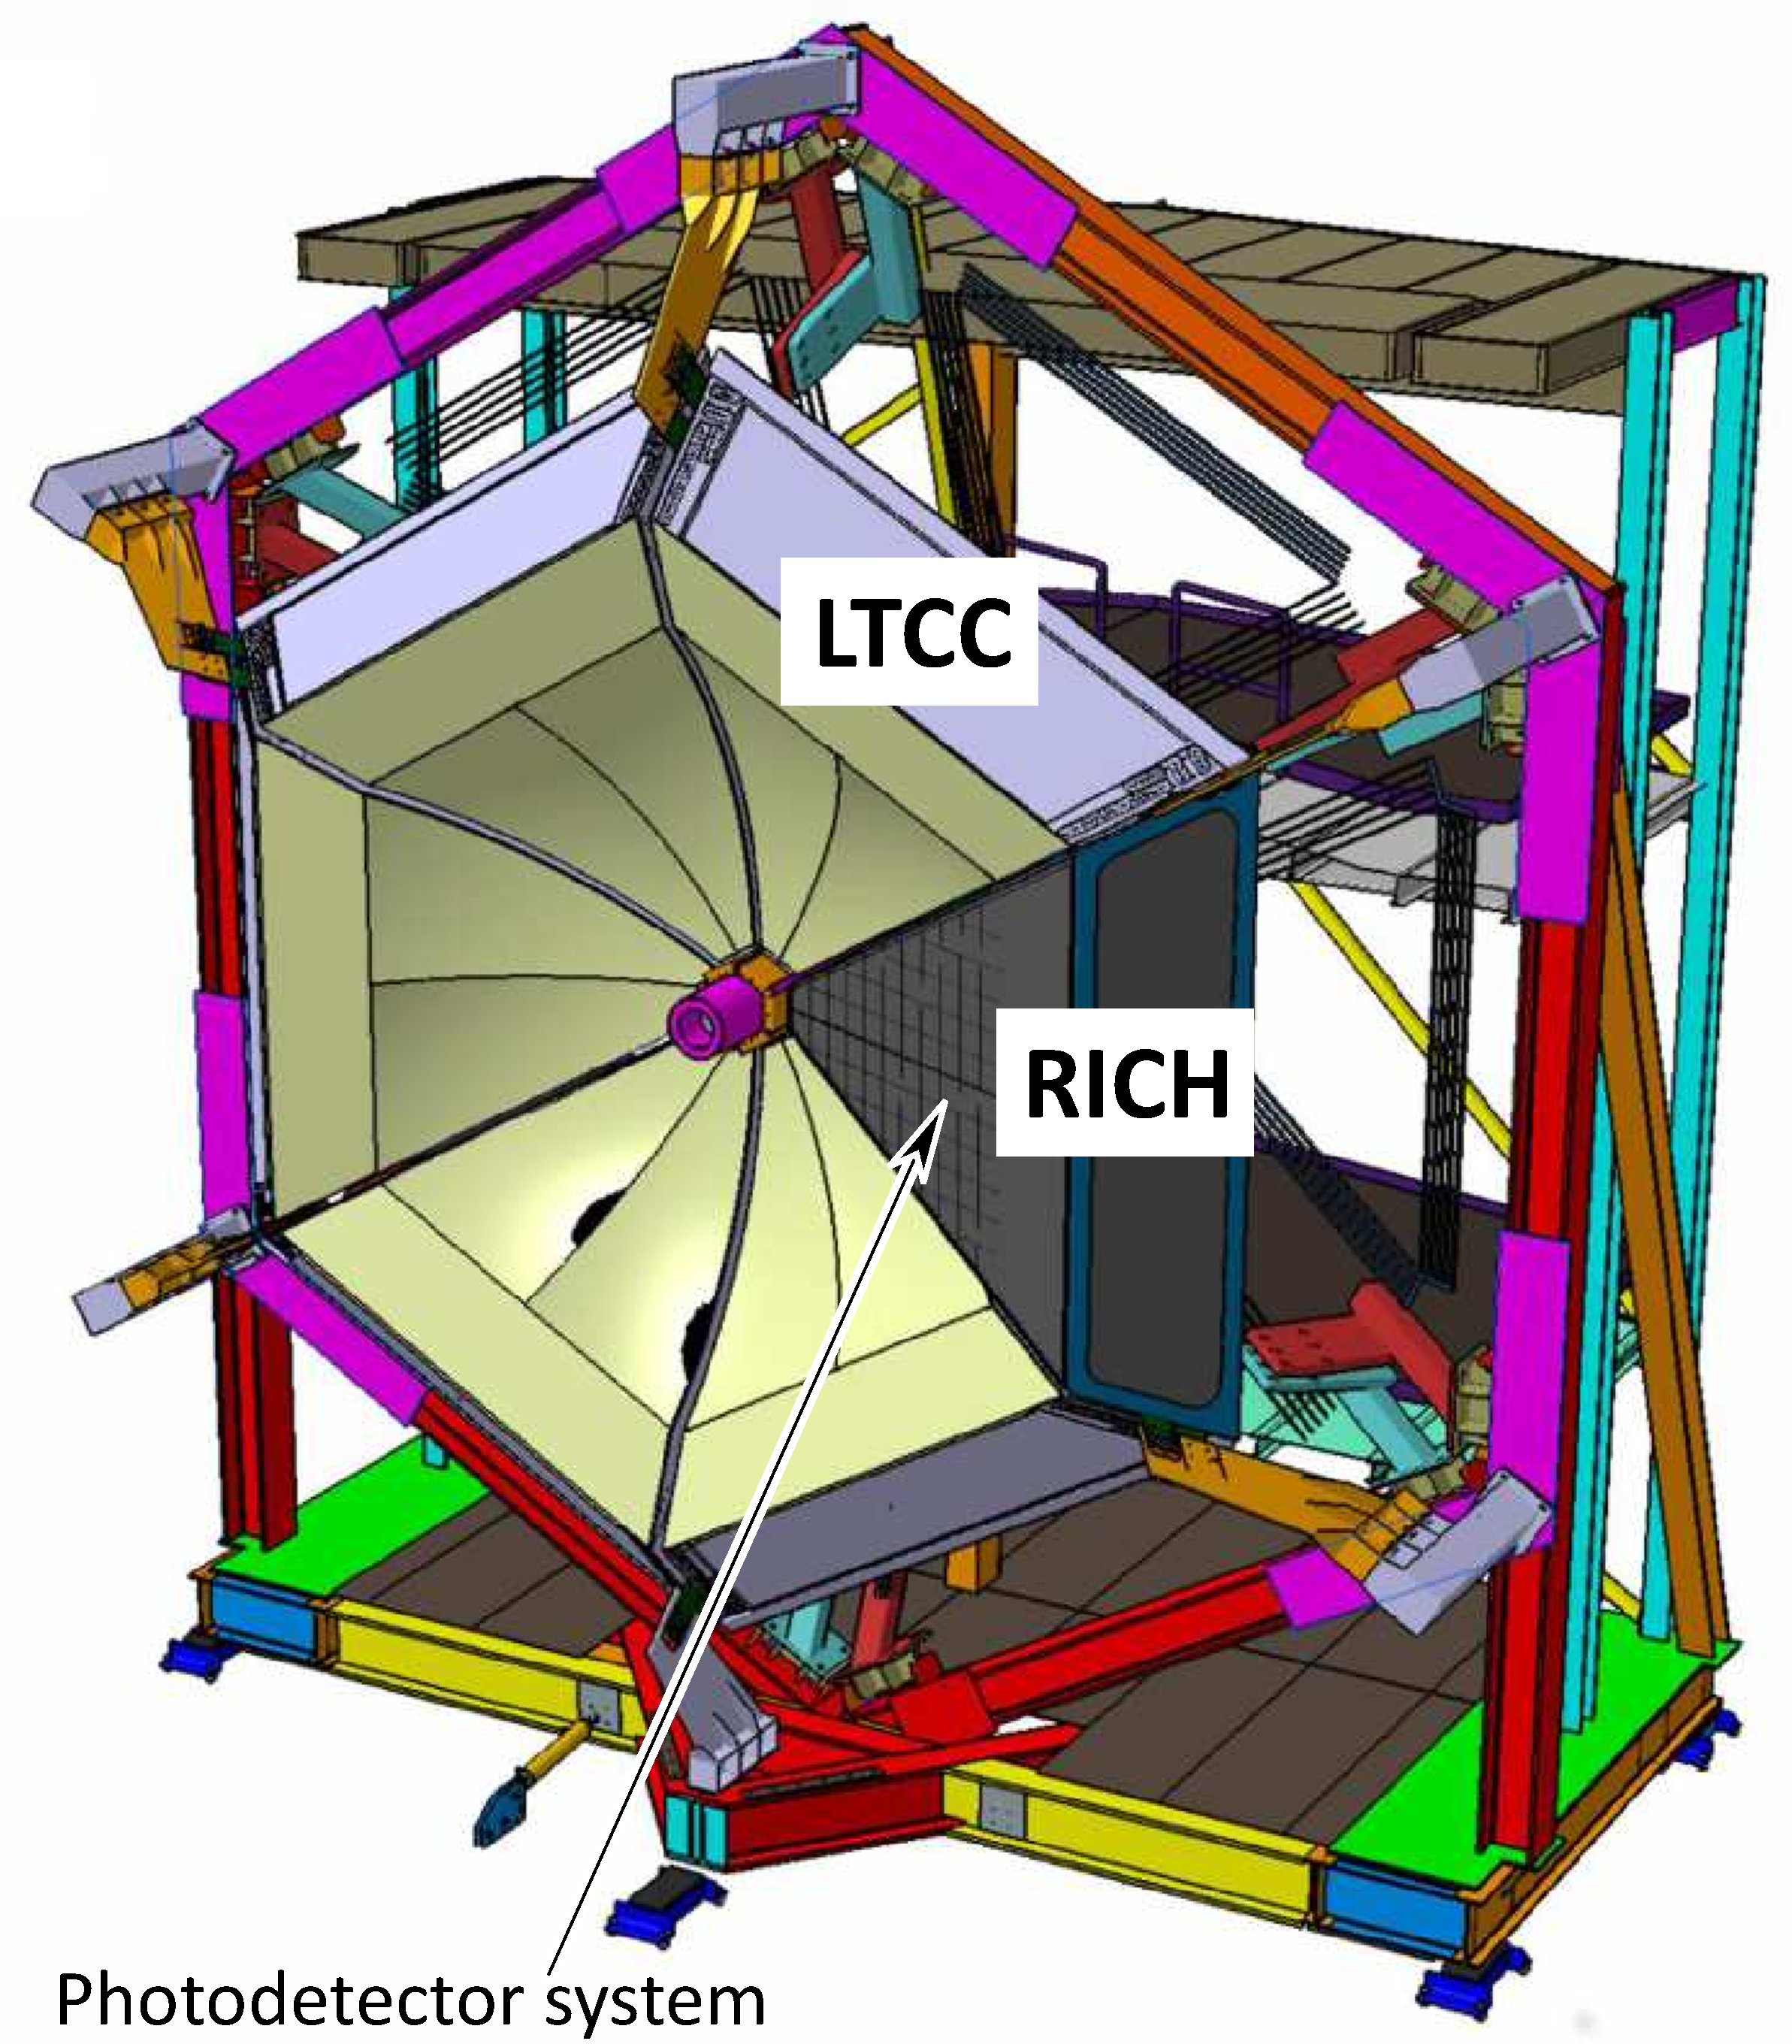
\includegraphics[width=0.7\linewidth]{RICHdetector.pdf}
	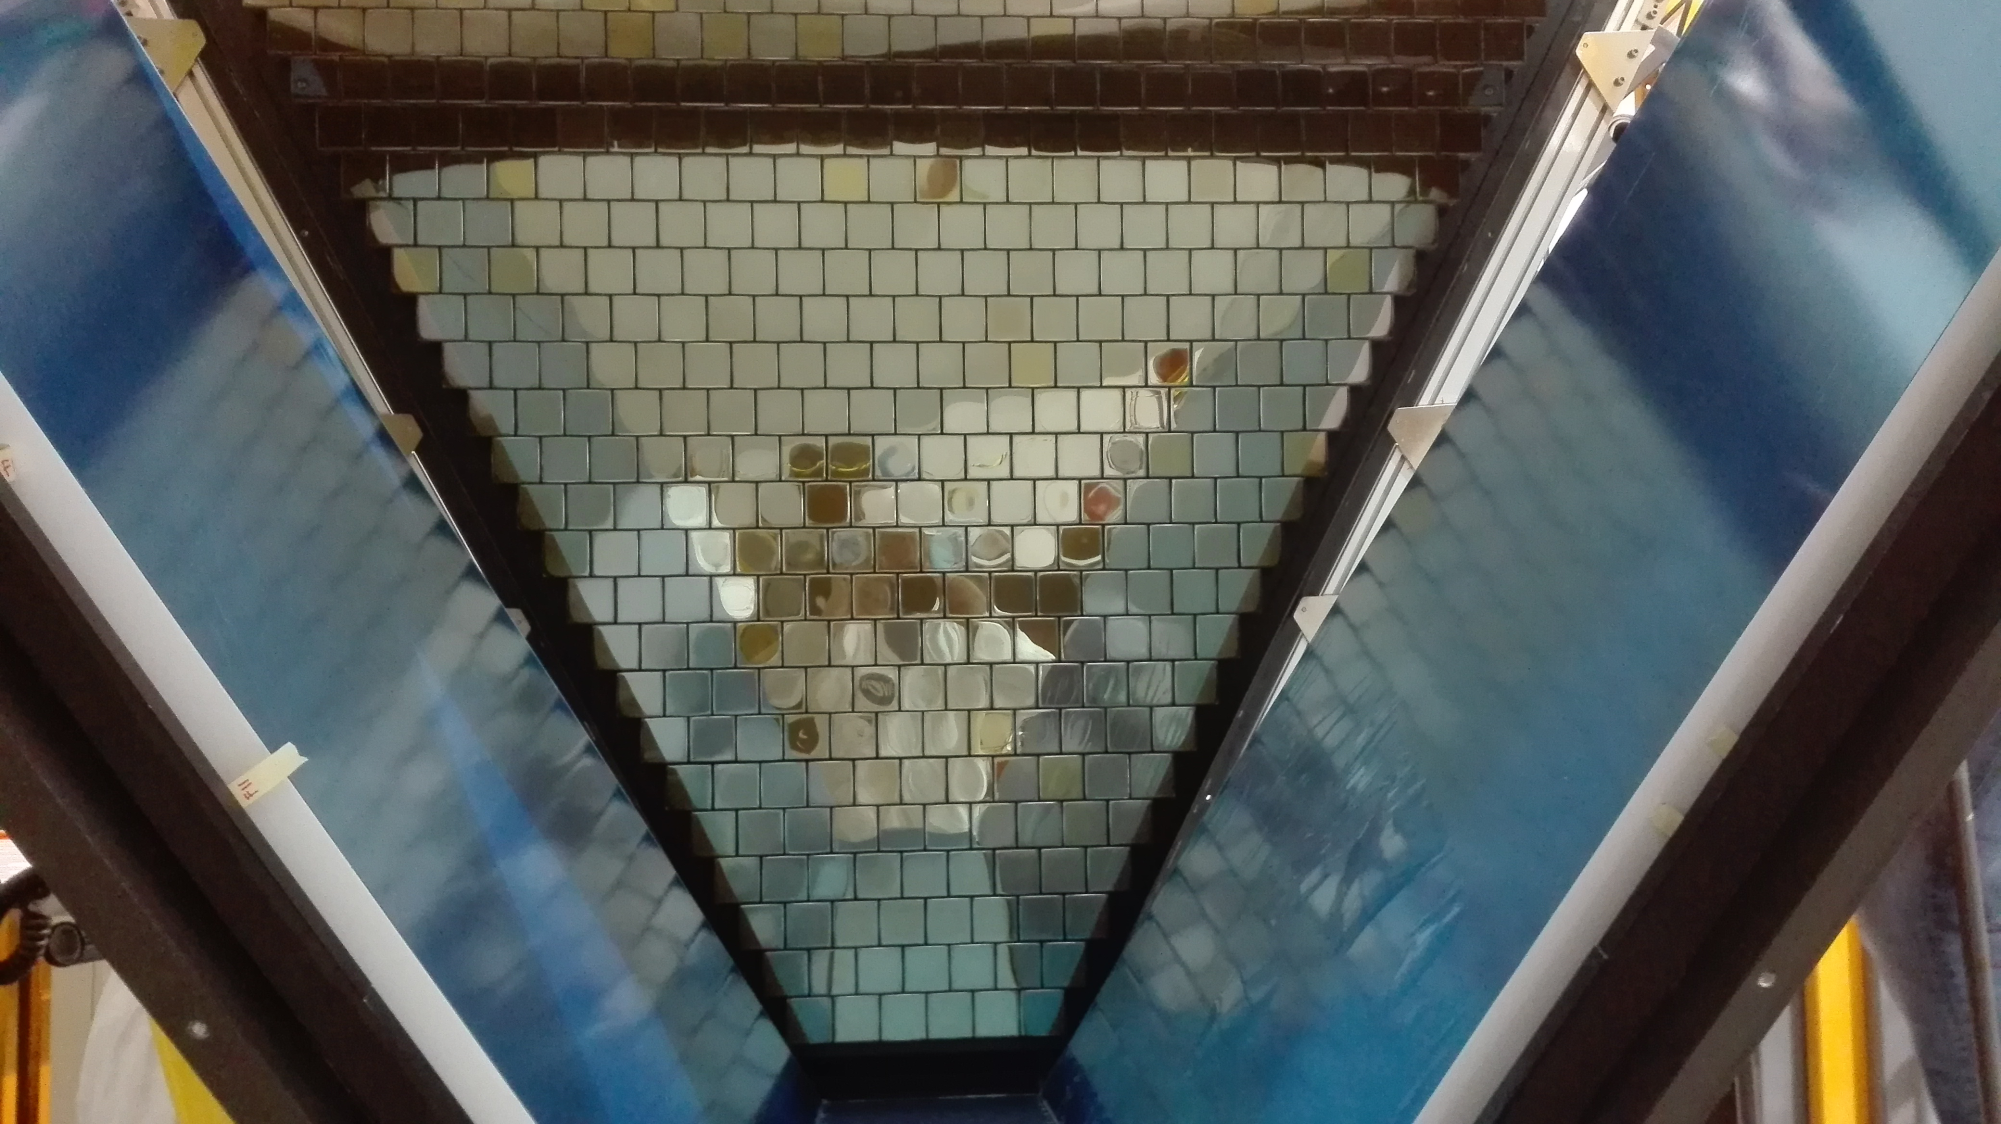
\includegraphics[width=0.7\linewidth]{RICHpanel_front.png}
	\caption{CLAS12 with RICH.}
	\label{fig:RICHdetector}
\end{figure}

The photon detector wall is a crucial component of the RICH detector (see Fig.~\ref{fig:RICHdetector}). It is relatively large and should be comprised of many photon detection devices such as photomultiplier tubes.
Due to the imaging aspect of the RICH they must provide a spatial resolution of less than 1 cm.
Since multiple photon detectors are tiled into large arrays, they should have large active area with minimal deadspace.
The photon detectors must also efficiently detect single photon level signals and should be sensitive to the visible light due to the aerogel radiator material.
Multi Anode PhotoMultiplier Tubes (MAPMTs) are perfect candidates for the CLAS12 RICH detector.
They are the flat-panel Hamamatsu MAPMTs offering an adequate compromise between detector performance and cost.
Each MAPMT comprises an 8 by 8 array of pixels,each with dimension of 6 by 6 mm.
Furthermore, the device has a very high packing fraction of 89\% with a high quantum efficiency in the visible light region.
The tubes also have excellent immunity to magnetic fields, because all internal parts are housed in a metal package and the distance between dynode electrodes are very short.


Initially, the Hamamatsu H8500 MAPMT model was chosen as the best option because they provide high quantum efficiency for visible light and sufficient spatial resolution (6x6 mm$^2$) at a limited cost.  However, recently Hamamatsu has released the new H12700 MAPMT model which shows enhanced single photoelectron (SPE) detection and is otherwise similar to the H8500 MAPMTs in spatial resolution, cost, and the rest.  Consequently we desire to better characterize the new H12700 MAPMTs and choose the best model between these two options for inclusion in the CLAS12 RICH.

These features pose challenging problem for the MAPMT testing and calibration.
RICH consists of 400 MAPMTs resulting in total number of channels equal to 25600. So in order to test them efficiently within a reasonable timeframe the fully automated test stand was build to evaluate 2 MAPMTs at once, with potential extension to 6 MAPMTs, as shown on Fig.~\ref{fig:MAPMTtest}.

\begin{figure}[hbt]
	\centering
	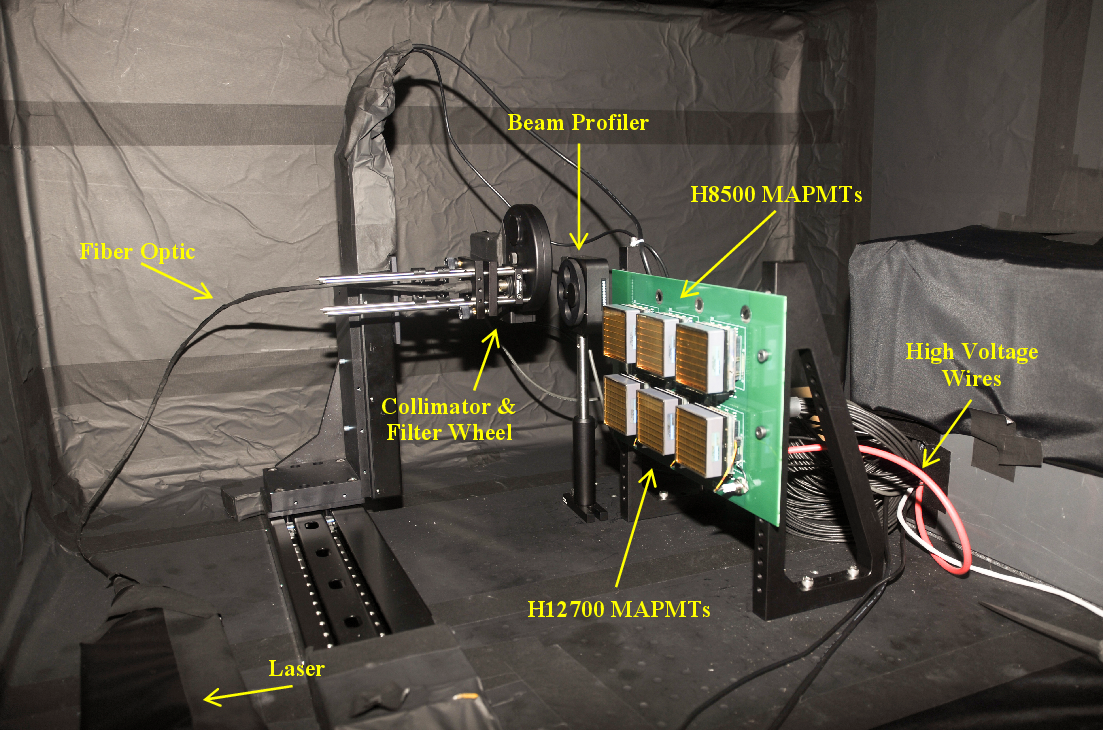
\includegraphics[width=0.9\linewidth]{blackbox.png}
	\caption{Evaluation setup.}
	\label{fig:MAPMTtest}
\end{figure}

The test stand consists of a 470 nm diode laser system, 2 long travel motorized stands to drive laser fiber in two dimensional space for individual pixel illumination, the motorized neutral density filter system, adapter board for MAPMT and JLab 250MHz FADC electronics for DAQ purposes.
The laser light is directed through the fiber and attenuated to the single photon level using the neutral density filters to mimic the conditions of the RICH detector.
The motors were remotely controlled to move the focused laser beam across (see Fig.~\ref{fig:beamopt1}) the entire surface of the MAPMT entrance window and illuminate one by one of all its 64 pixels individually.
Another option is to illuminate the whole surface of MAPMT photocathode at once using the Engineered Diffuser to produce square pattern with non-Gaussian intensity distribution (see Fig.~\ref{fig:beamopt2}).

\begin{figure}[bt]
	\centering
	\begin{subfigure}[b]{0.628\linewidth}
		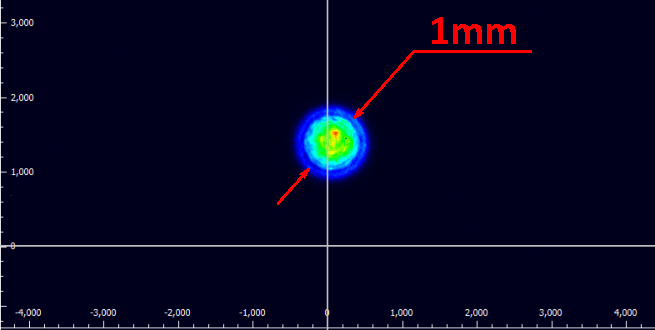
\includegraphics[width=\textwidth]{beamspot.pdf}
		\caption{Focused laser beam.}
		\label{fig:beamopt1}
	\end{subfigure}
	\begin{subfigure}[b]{0.354\linewidth}
		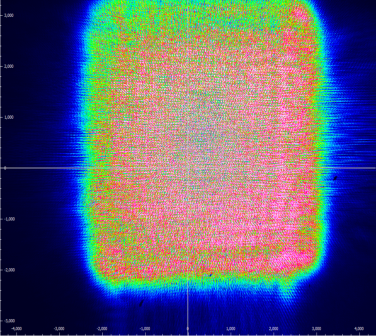
\includegraphics[width=\textwidth]{beamsquare.pdf}
		\caption{Square pattern.}
		\label{fig:beamopt2}
	\end{subfigure}
	\caption{The laser output options.}
\end{figure}

This configuration brings routine workload to minimum allowing the evaluation of 2 MAPMTs (equivalent to 128 conventional PMTs!) at 4 different high voltages and 6 different light intensities within 2 hours with less than 15 minutes of human intervention.

\begin{figure}[b]
	\centering
	\begin{subfigure}{0.3\linewidth}
		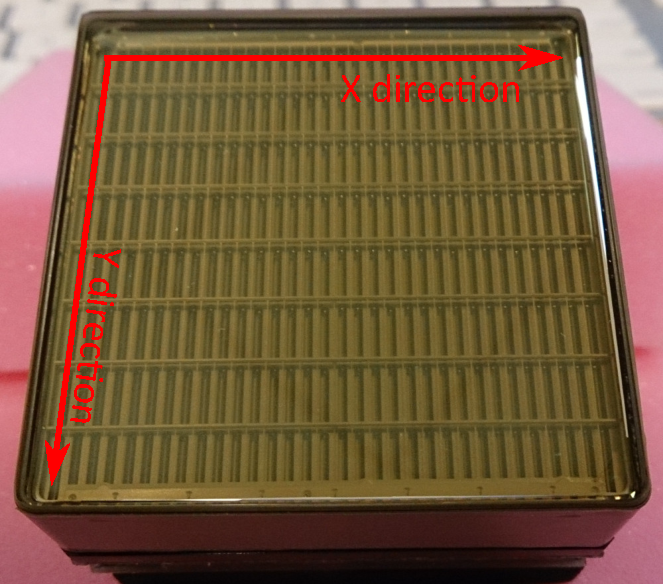
\includegraphics[width=\textwidth]{surfaceuniform1.pdf}
		\caption{MAPMT with visible internal structure of metal channel dynodes and focusing mesh.}
		\label{fig:surfaceuniform1}
	\end{subfigure}
	\quad
	\begin{subfigure}{0.3\linewidth}
		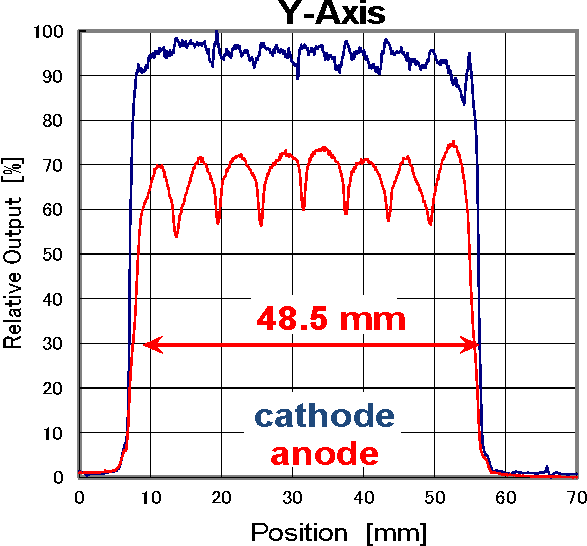
\includegraphics[width=\textwidth]{surfaceuniform3.pdf}
		\caption{The response along the X axis; the signal drops in the deadspace between the pixels.}
		\label{fig:surfaceuniform2}
	\end{subfigure}
	\quad
	\begin{subfigure}{0.3\linewidth}
		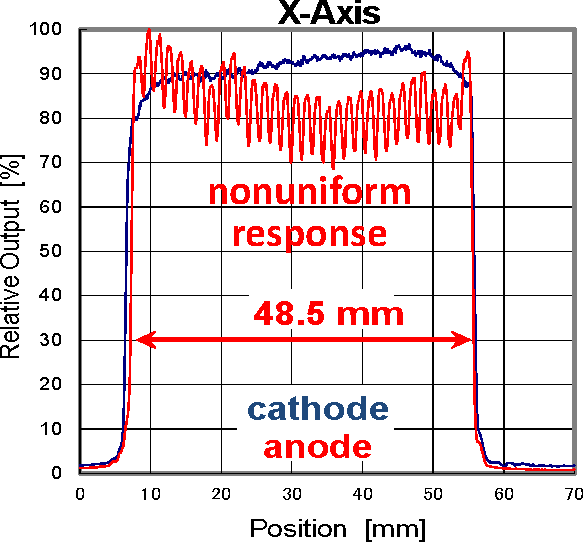
\includegraphics[width=\textwidth]{surfaceuniform2.pdf}
		\caption{The response along the Y axis: multiple segmentations within the pixels.}
		\label{fig:surfaceuniform3}
	\end{subfigure}
	\caption{The response uniformity of MAPMT.}
	\label{fig:surfaceuniform}
\end{figure}


Before starting the systematic study of the MAPMT responses, a finer two dimensional scan of several pixels was performed in order to verify the uniformity of the response across pixel's surfaces, as shown on Fig.~\ref{fig:surfaceuniform}.
The horizontal and vertical axes denote laser beam position during the scan.
Along the both directions there are obvious drops in efficiency when the laser strikes the space between the pixels.
The drops are relatively fast so the deadspace is very small as expected from the Hamamatsu specifications.
Additionally there exists a vertical efficiency variation across the pixel in horizontal scan.
These inhomogeneties are correlated with the vertical walls separating dynode chains, owing to the constructional features of the MAPMT. The discontinuity in dynode structure is visible from the MAPMT photon on Fig.~\ref{fig:surfaceuniform1}.
The separate response maps for photocathode shows relatively uniform signal without efficiency drops, confirming that the variation arises from the dynode system.



We started by using a model for signal amplitude distribution based off of Gaussian single photoelectron spectra as discussed in Bellamy et al. that works reasonably well for H8500, but this model does not satisfactorily treat the spectra seen in the new H12700 MAPMTs from Hamamatsu. Consequently, Pavel Degtyarenko~\cite{DEGTIARENKO20171} has developed a more complicated model using several Poisson components to better fit the MAPMT spectra, especially in the single photoelectron cases.
This mathematical model features a realistic descripription of the MAPMT response where each parameter corresponds to the physical process inside the MAPMT.
The SPE spectrum is fitted with a function used to describe the signal amplitude distribution measured by the MAPMT as shown on Fig.~\ref{fig:SPEfit},
The probability of an initial photon to knock out a photoelectron is distributed according to the Poissonian $P(m;\mu)=\frac{\mu^me^{-\mu}}{m!}$.
To approximate the performance of the first amplification cascade of the MAPMT the function $T(n,m;t)$ is introduced in the model as trinomial sum of three Poissonians with different average secondary multiplicities and the corresponding three relative probabilities for every photoelectron to generate secondary electrons.
The function $G(a,n;\sigma)$ corresponds to the realistic DAQ measurement function to introduce the experimental resolution into the resulting model function.

\begin{figure}[bt]
	\centering
	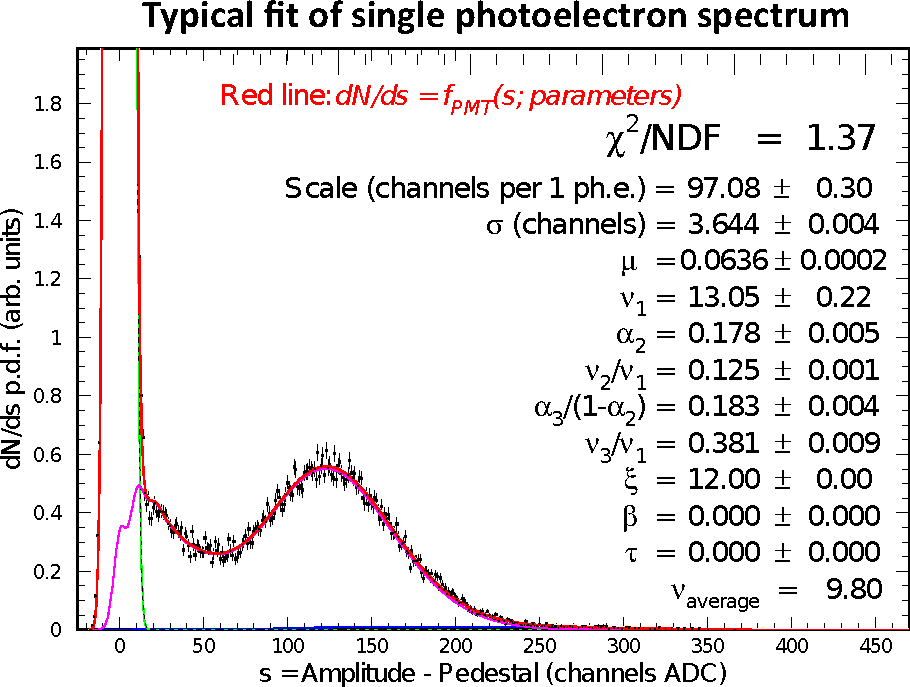
\includegraphics[width=\linewidth]{SPEfit.pdf}
	\caption{Sample of single photoelectron spectrum from one of the pixels at 1000 V with low intensity laser light source,
where integer $m$ corresponds to the number of photoelectorns created at the first stage of the photodetector (photocathode) by the incident light during one event of radiation, index $n$ corresponds to the number of electrons generated at the second stage of the photodetector (first dynode).
}
	\label{fig:SPEfit}
\end{figure}

The model is found to describe well the amplitude distributions measured at different levels of radiation with different supply voltages.
The parameters provide MAPMT characteristics independently of the test measurement conditions (see Fig.~\ref{fig:PavelPassport}): the $scale$ parameter is virtually independent on the light radiation level while strongly dependtnt on high voltage supply, the exact behavior one would expect from the characteristic of internal dynode system of MAPMT.

\begin{figure}[t]
	\centering
	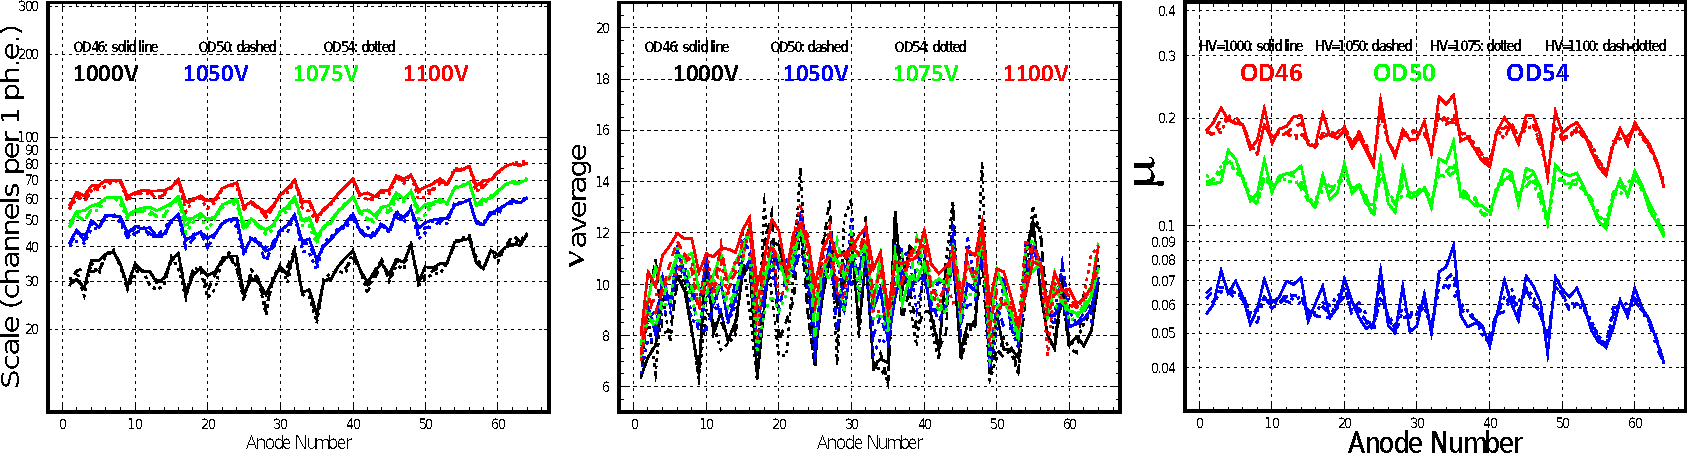
\includegraphics[width=\linewidth]{PavelPassport.pdf}
	\caption{Distributions of fit parameters among the pixels for measurements with 4 different high voltage supplies and 3 different light intensities: the parameter $scale$ characterizes the amplification (dynode) system, $\nu$ - first dynode performance, $\mu$ relates to the quantum efficiency (photocathode performance).}
	\label{fig:PavelPassport}
\end{figure}

Currently we have tested 80 H8500 and 260 H12700 (the largest collection of these new MAPMTs in the world).
The accumulated data provide an immense knowledge about quantum and collection efficiencies of MAPMTs, their surface uniformity, single photoelectron (SPE) spectrum resolution etc.
This parameterized information extracted from the fit of each pixel for every MAPMT is used to describe the detector response in the future simulation.



\begin{figure}[b]
	\centering
	\centering
	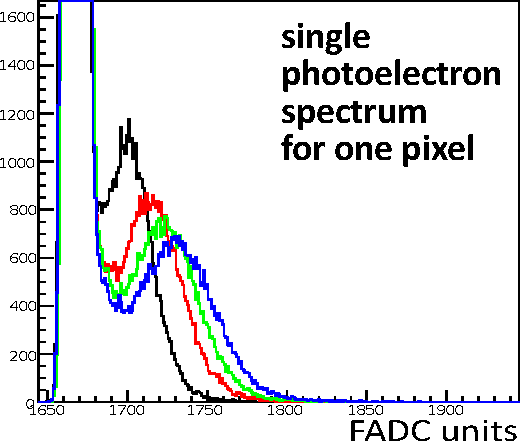
\includegraphics[width=0.8\linewidth]{SPEhv.pdf}
	\captionof{figure}{SPE spectra at 1000 (black), 1050 (red), 1075 (green) and 1100 (blue) V.}
	\label{fig:SPEhv}
\end{figure}

The performance of MAPMTs was evaluated under certain high voltages.
The single photoelectron spectrum and the pixel efficiency for H12700 MA-PMTs were tested and analyzed at 1000v, 1050v, 1075v, and 1100v.
The measurements performed at the reference supply voltage of 1000 V were compared to the measurements at different HV values in order to study the behavior of the MAPMT response as a function of the supply voltage.
As expected, it was found that the H12700 MA-PMTs perform the best in the single photoelectron spectrum efficiency at higher voltages, especially at 1100v.
We see a significantly improved separation of the first photoelectron peak from the pedestal at higher voltage supplies (see~Fig.~\ref{fig:SPEhv}).
When the average deficiencies of the tested MA-PMTs were analyzed, it was found that the average efficiency for 1000v, 1050v, 1075v and 1100v were approximately 4.6\%, 4.9\%, 5.0\%, and 5.2\%, respectively.
Therefore, the increase in detection efficiency is found to be over 10\% at 1100 V in comparison to 1000 V supply.
This separation is the crucial point for a single photon counting detectors such as CLAS12 RICH, where the occupancy is at the level of one photon per pixel.



It was also found that as the gain of the MAPMT increased, the efficiency ratio of 1100v to 1000v decreased.
The ratio is shown on~Fig.~\ref{fig:effratio} as a function of MAPMT gain reported by Hamamatsu.
The high voltage supply improves the performance of MAPMT dynode system, decreasing the fraction of the single photoelectron events below the pedestal peak.
This indicates that lower gain MAPMTs have a greater difference in the efficiencies at 1100v and 1000v, while higher gain MAPMTs have a smaller difference between the two voltage efficiencies.
The improvement for lower gain MAPMTs is more significant than for higher gain MAPMTs, because the high gain MAPMT has good separation of signal from pedestal even at the reference 1000 V.
Therefore, the low gain MAPMT benefit greatly from higher supply voltage.
The collected data are used to determine what high voltage the MAPMTs should be ran at to acquire the best results when the RICH detector is completed.


\begin{figure}[bt]
	\centering
	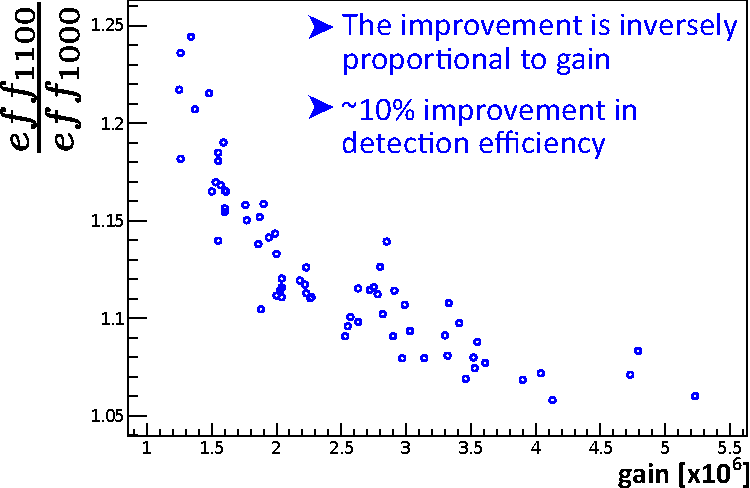
\includegraphics[width=0.8\linewidth]{effratio.pdf}
	\caption{Ratio of MAPMT efficiencies at 1100 and 1000 V as a function of MAPMT gain.}
	\label{fig:effratio}
\end{figure}

The parameters from Pavel's PMT response function are shown on the Fig.~\ref{fig:mu} and \ref{fig:characteristicPars} and correspond to the emission of the photoelectron ($\mu$), its collection and multiplication on the first dynode ($scale$ and $\nu$).
We have omitted other parameters that take into account the resolution effects of readout system or correspond to the cascade multiplication of the secondary electrons as they are out of scope focus of our analysis.
Given our requirements for single photoelectron signal sensitivity MAPMTs of our choice should be able to detect with high probablity single photon that reaches photocathode.
In order to achieve this goal MAPMT should have high quantum efficiency of the photocathode as well as high collection efficiency of produced photoelectron combined with substantial signal multiplication to achieve good resolution of SPE peak.
These characteristics were studied in bulk for all 27520 channels (430x64) during the different light conditions and for different supplied HV values.

\begin{figure}[bt]
	\centering
	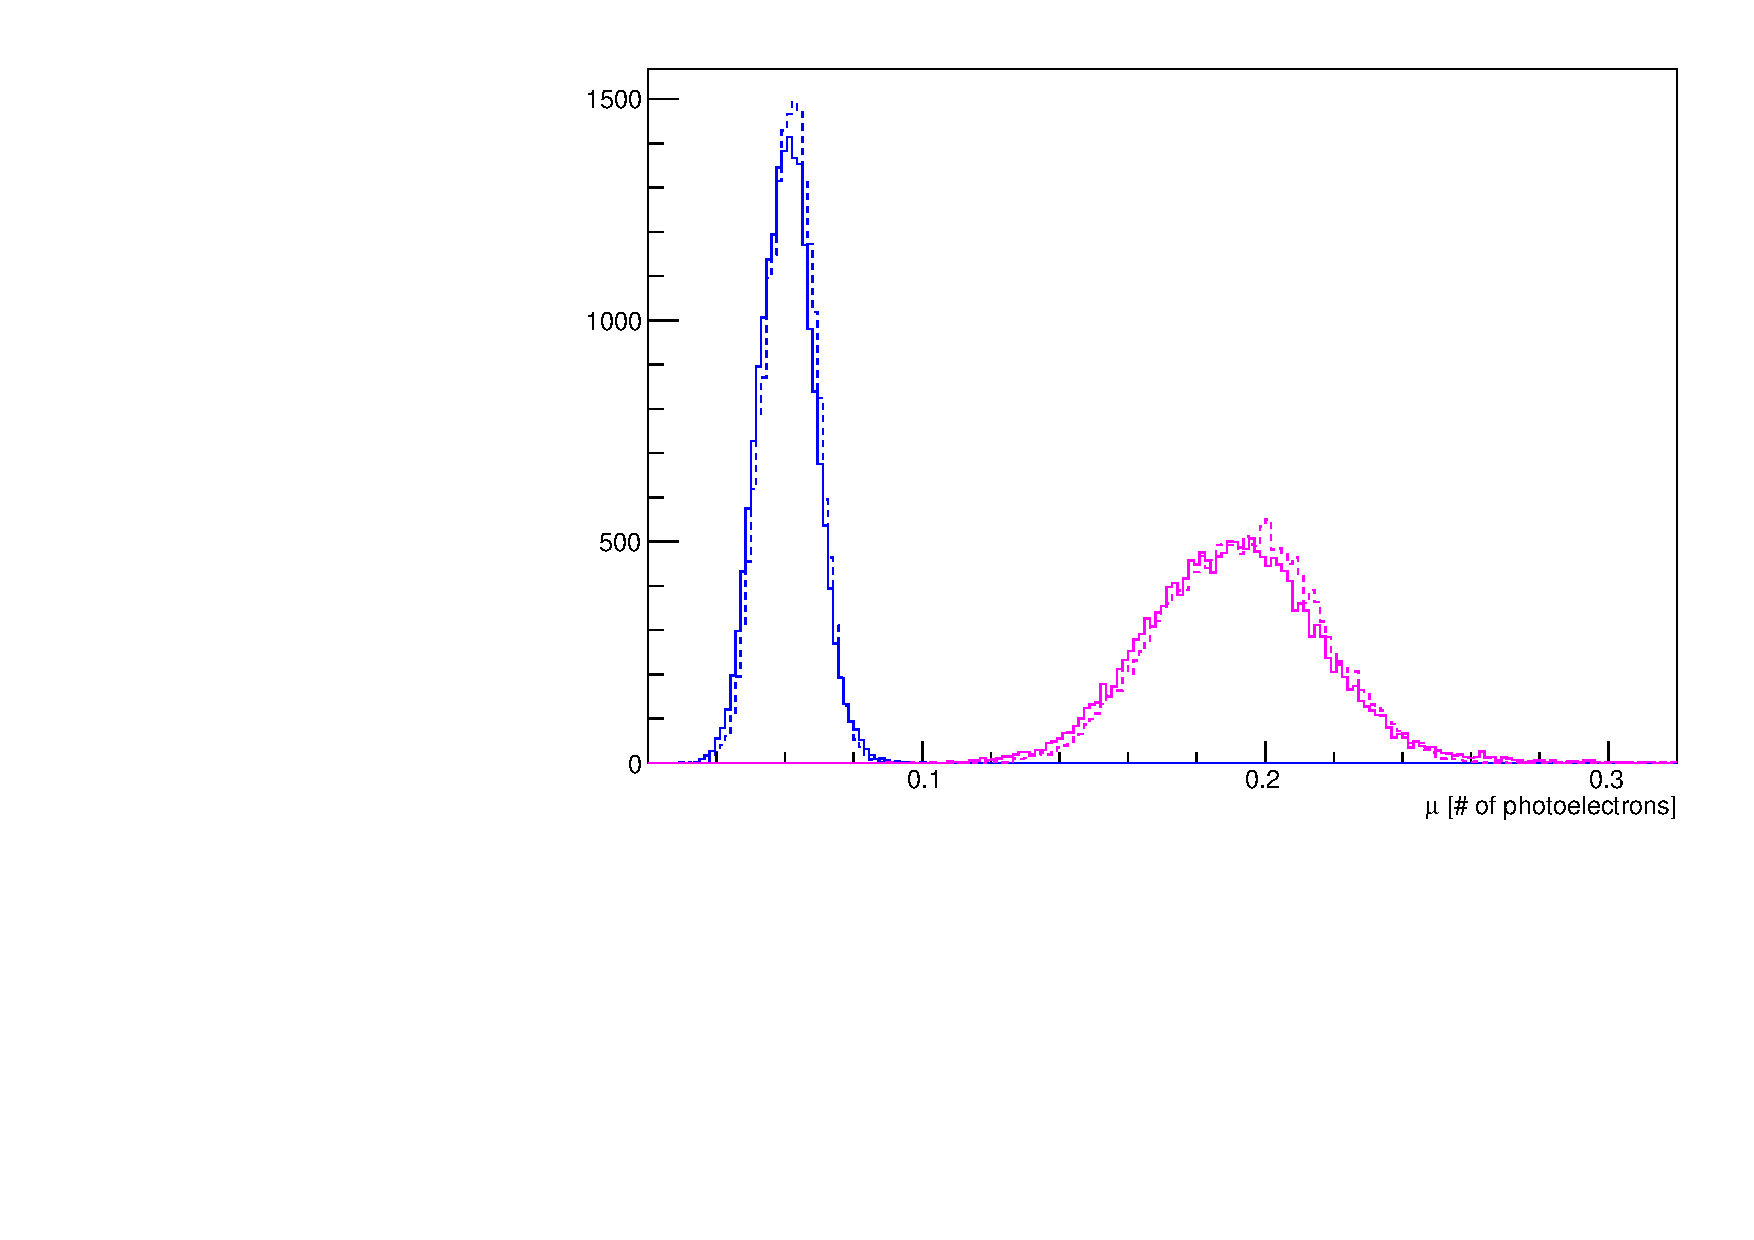
\includegraphics[width=0.8\linewidth]{mu.pdf}
	\caption{Average number of the photoelectrons emitted from the photocathode for different laser light intensities: $10^{-5.4}$ - blue and $10^{-4.6}$ - red. Solid line is for measurements at 1000 V and dashed - at 1100 V}
	\label{fig:mu}
\end{figure}

Fig.~\ref{fig:mu} shows the distribution of parameter $\mu$ which correspond to the average number of the photoelectrons produced during the measurements.
This parameters represents the convolution of the MAPMT photocathode quantum efficiency and laser setup light intensity.
Both characteristics should not depend on HV supply values and it is demonstrated on this figure by comparison of $\mu$ values extracted for the measurements at 1000 V and 1100 V.
However one can change the parameter by varying the laser light intensity which is evident from the left shift of $\mu$ values for lower light intensity measurements.

The other two free parameters are plotted on Fig.~\ref{fig:characteristicPars}.
They correspond to the average number of second-stage electrons produced on the first dynode by photoelectron (see~Fig.~\ref{fig:nu} and average signal amplitude for single photoelectron spectrum (see Fig.~{fig:scale}).
Both parameters characterize mainly the amplifying subsystem of MAPMT and therefore should depend on supplied HV.
The measurements at 1000 V and 1100 V confirm that amplification is improved at higher values of applied high voltage.
Traditionally the second parameter (gain) is often used to describe the amplification abilities of photomultipliers and often used in calibration and reconstruction procedures.
And it was shown that the extracted gains do not depend on the light conditions with a high degree of accuracy.

\begin{figure}[b]
	\centering
	\begin{subfigure}{0.48\linewidth}
	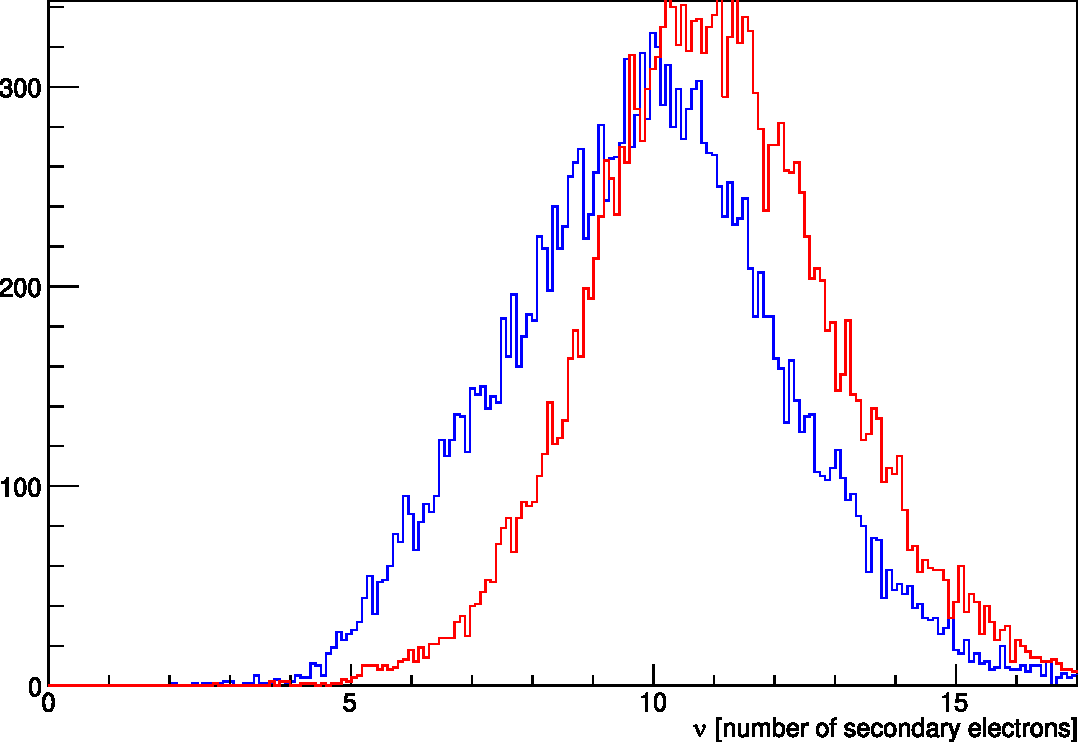
\includegraphics[width=\linewidth]{nu.pdf}
	\caption{}
	\label{fig:nu}

	\end{subfigure}
	\begin{subfigure}{0.48\linewidth}
	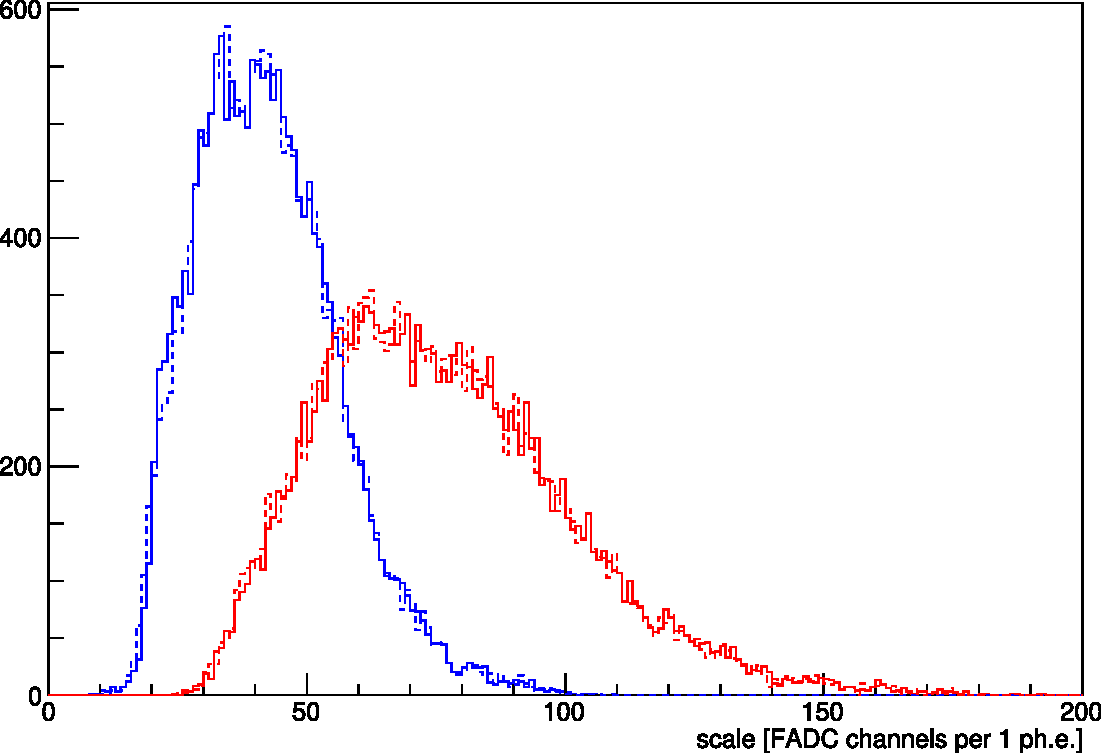
\includegraphics[width=\linewidth]{scale.pdf}
	\caption{}
	\label{fig:scale}
	\end{subfigure}

	\caption{Characteristic parameters of single photoelectron signal distributions from Hamamatsu H12700 MAPMT in the framework of Pavel Degtiarenko's model for measurements at different HV: 1000 V (blue) and 1100 V (red):
		(a) average number of second-stage electrons knocked out of the first dynode,
		(b) the average signal amplitude per single photoelectron for different light intensity measurements: at $10^{-5.4}$ (solid line) and at $10^{-4.6}$ (dashed) attenuation}
	\label{fig:characteristicPars}
\end{figure}





\section{Results}

We saw that although there is little difference in crosstalk signals, the H12700 PMTs suffer less from dark current, have narrower SPE spectra, and have higher $\mu$ and relative efficiency values.
%An example plot of the $\mu$'s and relative efficiencies of H8500 and H12700 PMTs with similar low and high gains is shown in Figure \ref{efficiency}.


We see that the relative efficiency is closely related to the $\mu$ which is on average, over all pixels at all voltages for all the PMTs we tested, $29\pm5$ percent higher in H12700 than H8500 MAPMTs. One concern with these $\mu$ measurements however is that the laser system used to measure these PMTs was only incident on a portion of each pixel, consequently missing their sum total effect and pinpointing possible spatial dependencies which should be further studied and perhaps remeasured with a fully illuminated MAPMT instead of collimated pinpoint laser light. In terms of crosstalk for the two varieties of MAPMT the H12700s appear to be better than the H8500s. The H12700s have a decrease in crosstalk by nearly a factor of two. Additional studies of dark current in the H12700s would be useful, as the dark current is usually dominated by individual pixels or bad regions of the PMT instead of spread around evenly like in the H8500s, but overall the two varieties are not very different in terms of dark current.

\bibliographystyle{elsarticle-num-names}
\bibliography{bib_vpk}


\end{document}
